\documentclass{beamer}

\usepackage{multicol}
\usepackage{float}
\usepackage{lmodern}

\usetheme[progressbar=frametitle]{metropolis}
\setbeamertemplate{frame numbering}[fraction]
\useinnertheme{metropolis}
\useoutertheme{metropolis}
\usefonttheme{metropolis}
\usecolortheme{spruce}
\setbeamercolor{background canvas}{bg=white}
%different themes are available
\definecolor{babyblueeyes}{rgb}{0.63, 0.79, 0.95}
%define custom theme using rgb, check latexcolor.com for information
\usecolortheme[named=babyblueeyes]{structure}


% Python style for highlighting
\usepackage[utf8]{inputenc}

% Default fixed font does not support bold face
\DeclareFixedFont{\ttb}{T1}{txtt}{bx}{n}{12} % for bold
\DeclareFixedFont{\ttm}{T1}{txtt}{m}{n}{12}  % for normal

% Custom colors
\usepackage{color}
\definecolor{deepblue}{rgb}{0,0,0.5}
\definecolor{deepred}{rgb}{0.6,0,0}
\definecolor{deepgreen}{rgb}{0,0.5,0}
\definecolor{almostwhite}{rgb}{0.99,0.99, 0.99}

\usepackage{listings}

% Python style for highlighting
% Check out how to use minted next time
% Seems simpler

%Frame title command
\newcommand{\floattitle}[1]{%
	\begin{beamercolorbox}[sep=0.3cm,left,wd=\paperwidth]{frametitle}
		\usebeamerfont{frametitle}%
		\vbox{}\vskip-1ex%
		\strut#1\strut\par%
		\vskip-1ex%
	\end{beamercolorbox}%
}

\lstset{
	basicstyle  =   \footnotesize,
	keywordstyle    = \color{deepred}\bfseries,
	stringstyle     = \color{strings},
	identifierstyle = \color{black},
	commentstyle    = \color{deepgreen},
	breaklines=true,
	numbersep=-10pt,
	stepnumber=1,
	showspaces=false,
	escapechar=§,
	showstringspaces=false,
	showtabs=false,
	frame=single,  
	rulecolor=\color{black},
	tabsize=4,              
	captionpos=t,           
	breaklines=true,
	breakatwhitespace=false,
	numbers=left,
	extendedchars=\true,
	emph=[3]{href, Particle, Boris_update, Field, uniform_E_field, radial_E_field, uniform_B_field, helmholtz_coil_B_field, two_helmholtz_B_field, Sampler, sample_uniform_position, sample_uniform_velocity, sample_velocity_uniformKE, sample_Maxwellian_velocity, sample_parabolic_velocity},
	emphstyle=[3]{\color{deepblue}},
	backgroundcolor=\color{almostwhite},
	language=Python 
}

%until here


\title[]{Magnetic Mirror Effect in Magnetron Plasma:}
\subtitle{Modeling of Plasma Parameters}


%may use macros to set new frame defaults

\setbeamercovered{transparent=25}
%hide onslide part by making it more transparent
%cant do this with only, but with onslide


\newcommand\myfigure[1]{%
	\medskip\noindent\begin{minipage}{\columnwidth}
		\centering%
		#1%
		%figure,caption, and label go here
	\end{minipage}\medskip}
\newcommand{\comment}[1]{}

\begin{document}
	\metroset{block=fill}
	%shades the background of a block
	
	%In beamer we create frames 1 frame= 1 page to hold our information
	\begin{frame}
		\fontfamily{ppl}\selectfont 
		\begin{center}
			\large{\textbf{MEE4099 Capstone Project}} \\ 
			\normalsize{Review 1 tentative presentation: first draft} \\
			\normalsize{Project Title:} \\ 
			\Large{\textbf{Magnetic Mirror Effect in Magnetron Plasma:}} \\
			\Large{\textbf{Modeling of Plasma Parameters}} \\
		\end{center}
		%\color{blue}
		\textbf{Project ID:} 21BTECH10051 \\
		\textbf{Team Members:} \\
		18BEM0145 Sashi Kant Shah \\
		18BME2104 Kaushal Timilsina \\
		18BME2109 Hrishav Mishra \\
		
		\noindent \textbf{Internal Guide:} \\
		Professor Sitaram Dash	
	\end{frame}	

	\section{1. Introduction}
	\begin{frame}[allowframebreaks]
		\floattitle{1.1 Plasma}
		Non equilibrium state with long range dynamics \\
		
		\begin{enumerate}
			\item Number density, $n$ \\
			Number of particles per unit volume. \\
			Mass density $\varrho := m n$ \\ $m$ is the mass of particles of the species.
			
			\item Ionization, $\alpha$ \\
			$\alpha := \frac{\displaystyle n_{charged}}{\displaystyle n_{charged} + n_{neutral}}$ \\
			$\alpha = 1$: all the particles are charged \\ $\alpha = 0$: all the particles are neutral
			
			\item Temperature, $T$ \\
			describes the average kinetic energy of the particles in the plasma
			
			\item Mean free path, $\lambda_{mfp}$ \\
			influenced by the temperature \\
			$\lambda_{mfp} := v_{th} \tau$ \\
			$v_{th}$: thermal velocity of the particles \\ $\tau$: timescale of collisions. 
			
			\item Plasma beta parameter\\
			$\beta := \frac{\displaystyle 8 \pi n T}{\displaystyle B^{2}}$ \\ 
			ratio of the thermal and magnetic energies of the plasma\\ 
			random thermal motions compete with the Lorentz force.
			
			\framebreak
			
			\item Debye Length, $\lambda_{D}$ \\
			\textbf{Competing}
			\begin{multicols}{2}
				Coulumb interactions \\
				between charged particles \\
				\columnbreak
				Random thermal speed \\
				based on temperature
			\end{multicols}
			\textbf{Debye sphere}:
			imaginary sphere around a charged particle \\
			where oppositely charged particles are attracted \\
			screen the charge of the central particle to the outer plasma \\
			electrostatic influence of a particle is limited to the Debye sphere surrounding it\\
			\textbf{Quasi-neutral behavior}: \\
			electrostatically neutral on scales $>\lambda_{D}$. \\
			Debye length, $\lambda_{D}$: radius of the Debye sphere.
			
			Other parameters: Larmor radius, frequencies of waves, etc.
		\end{enumerate} 
		
		
	\end{frame}

	\begin{frame}[allowframebreaks]
		\floattitle{1.2 Laboratory Plasma}
		Properties of laboratory plasma
		\begin{itemize}
			\item High ionization fraction
			\item Sub atmospheric pressure required to sustain ionization
			\item Temperature range : 1000 - 30000 K
		\end{itemize}
		
		\noindent Surface engineering techniques that use plasma
		\begin{enumerate}
			\item Plasma Immersion Ion Implantation (PIII)
			\item Plasma Enhanced Chemical Vapor Deposition (CVD)
			\item Magnetron Sputtering (PVD)
			\item Air Plasma Spray (Spray technique)
			\item Plasma Transferred Arc (Hardfacing technique)
		\end{enumerate}
	\end{frame}

	\begin{frame}[allowframebreaks]
		\floattitle{1.3 Physical Vapor Deposition}
		Thin film coatings are grown on the surface of a specimen \\
		Random walker particles get trapped in strained pockets\\ Produce nucleation site
		\begin{enumerate}
			\item Sputtering techniques \\
			\textbf{Cold techniques}\\
			high energy beam removes material from a target\\
			removed material is coated on the substrate.
			
			\item Evaporation techniques \\
			\textbf{Hot techniques}\\
			heating the material to  to a high temperature \\ particles in the vapor are coated on the substrate\\
			Semiconductors like Si/Ge, insulators like oxides and metals like Tungsten often coated 
		
		\end{enumerate}
	\end{frame}
	
	\begin{frame}[allowframebreaks]
		\floattitle{1.4 Magnetron sputtering}
		Sputtered ions form a magnetically confined plasma\\
		Plasma controlled by magnetic fields\\ 
		Transports ions to the surface of the substrate forming the coating. 
		
		\begin{figure}[H]
			\phantom{text}
			\begin{center}
				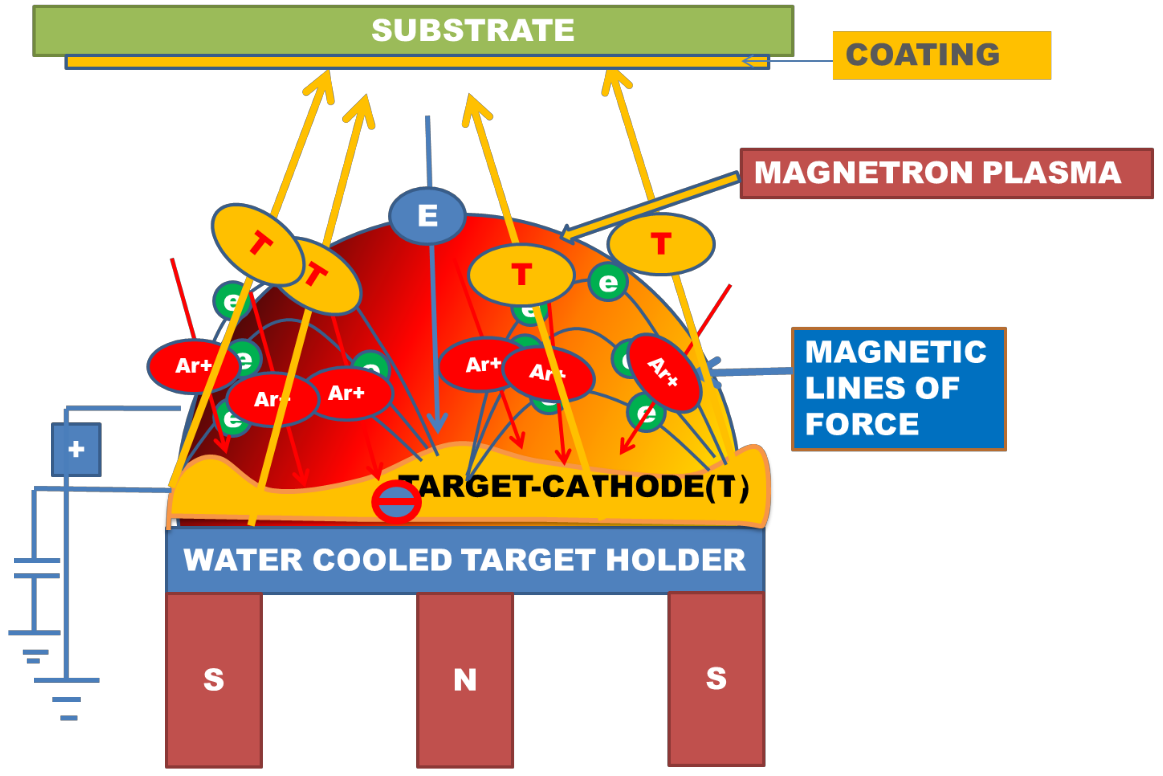
\includegraphics[width=10cm, height=7cm]{magnetron sputtering.png} \caption{Magnetron Sputtering system. credit: \cite{SurfaceEng}}
			\end{center}
		\end{figure}
	\end{frame}

	\begin{frame}[allowframebreaks]
		\floattitle{1.5 Magnetic Mirror}
		a
	\end{frame}
	
\begin{frame}[allowframebreaks]
	\begin{thebibliography}{}
		\floattitle{References}
		\bibitem{SurfaceEng}
		Professor Sitaram Dash. (Fall Semester 2021). \textit{MEE4005 Surface Engineering} (lecture notes). SMEC, VIT Vellore.
		\bibitem{MKunz}
		Matthew W. Kunz. (November 9, 2020). \textit{Introduction to Plasma Astrophysics} (lecture notes). Princeton Plasma Physics Laboratory.
		\bibitem{chenbook}
		Chen, F. F. (1984). \textit{Introduction to plasma physics and controlled fusion} (Vol. 1, pp. 8-11). New York: Plenum press.
		\bibitem{mirror1}
		Na, Yong-Su (2017). \textit{Introduction to nuclear fusion} (Lecture 9 Mirror, lecture slide). Seoul National University Open Courseware.
		\bibitem{mirror2}
		F\"{o}rel\"{a}sning (2009). \textit{Charged particle motion in magnetic field} (lecture slide). Lule\"{a} University of Technology.
		\bibitem{PIC good}
		Myers, A., Colella, P., \& Straalen, B. V. (2017). \textit{A 4th-Order Particle-in-Cell Method with Phase-Space Remapping for the Vlasov--Poisson Equation}. SIAM Journal on Scientific Computing, 39(3), B467-B485.
		\bibitem{PIC IAS}
		Anatoly Spitkovsky (2016). \textit{Kinetic plasma simulations} (lecture slide). PiTP 2016 on Computational Plasma Astrophysics. Institute for Advanced Study.
		\bibitem{Borisgood}
		Qin, H., Zhang, S., Xiao, J., $\&$ Tang, W. M. (April, 2013). \textit{Why is Boris algorithm so good?}. Princeton Plasma Physics Laboratory, PPPL-4872.
		
	\end{thebibliography}
\end{frame}

\end{document}